% l	&	\underbrace{\red{\D u\left(x_n\right)}\strut}_{\text{function of Wealth}\strut} 	&	\cdot
% 	&	\underbrace{p_n\strut}_{\text{objective probability}\strut}  \\
% 	%
% 	\elabel{EvoDTs3}
% 	&	\text{Cumulative Prospect Theory:} &\mathfrak{V}\left( f_X \right)
% 	&=	\sum_{n=1}^{\infty} & \underbrace{\red{\mathfrak{v}\left(\Dx_n\right)}\strut}_{\text{function of the payout}\strut} &	\cdot &	\underbrace{\blue{\pi\left(p_n\right)}\strut}_{\text{function of obj. probability}\strut}
% \end{align*}
% 
% % \vfill
% 
% \gray{\footnotesize $x$ wealth, $\Dx$ payout, $p$ probability, $u$ utility function, $\mathfrak{V}$ value/prospect,\\
% $\mathfrak{v}$ value function, $\pi$ probability weighting, $f_X$ lottery/probability mass function of a random variable}
% 
% \label{EvolutionDT}
% 
% % \framebreak
% % 
% % \begin{align*}
% %  \elabel{EvoDTsEDU}
% % 	&	\text{Expected discounted utility:} &\EA{\beta^t\Du\left(X\right)}	&= \sum_{n=1}^{\infty}
% % 	&	\underbrace{\blue{\beta^t \D u\left(x_n\right)}\strut}_{\text{function of Wealth}\strut} 	&	\cdot
% % 	&	\underbrace{p_n\strut}_{\text{objective probability}\strut}  \\
% % 	%
% % 	\elabel{EvoDTsBUT}
% % 	&	\text{Behavioural Utility:} &\mathfrak{V}\left( f_x \right)
% % 	&=	\sum_{n=1}^{\infty} & \underbrace{\blue{\mathfrak{v}\left(\Dx_n\right)}\strut}_{\text{function of the payout}\strut} &	\cdot &	\underbrace{\blue{\pi\left(p_n\right)}\strut}_{\text{function of obj. probability}\strut}
% % \end{align*}
% 
% \end{frame}


% \section[Probability Weighting]{What are weighting for? A mechanistic explanation of probability weighting}
\section{Main Result}

\begin{frame}{Main result}
\begin{center}
\only<1->{
	\includegraphics[width=.45\textwidth]{../figs/KT_result_nolegend.pdf}
	}
\uncover<2>{
\includegraphics[width=.45\textwidth]{../figs/Our_result_nolegend.pdf}
	}
\end{center}

% \begin{enumerate}
% 	\item	inverse-S shape can be explained by difference in uncertainty
% 	\item cautious estimation of probabilities generates such differences
% % 	\item	relative estimation error in $p(x)$ is greater for rarer events 	
% \end{enumerate}
\label{MainResults}
% \hyperlink{weight_vs_estimate}{\beamergotobutton{PW K\&T 1979}}
\end{frame}

% \begin{frame}{Agenda}
%  \tableofcontents[hidesubsections]
% \end{frame}

\section{Probability Weighting}

\begin{frame}{Definition of Probability Weighting (PW)}

\begin{columns}%[T]
\column{0.5\textwidth}
% {\centering	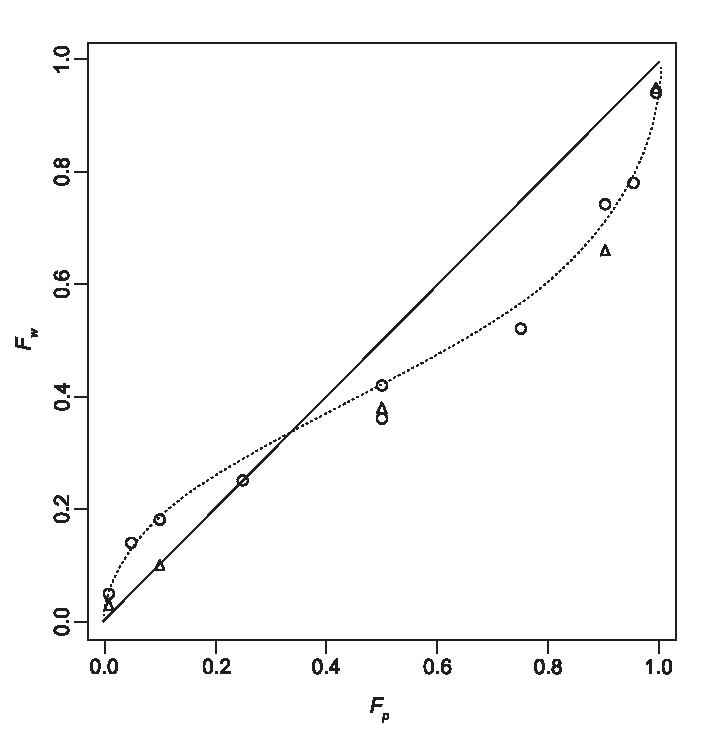
\includegraphics[width=.9\textwidth]{../figs/TK1992.pdf} }
% \parencite[p. 310, Fig. 1,relabelled axes]{TverskyKahneman1992}
{\centering	\includegraphics[width=.9\textwidth]{../figs/PB48_connectedDots.pdf} }
\parencite[p. 188, Fig. 1, relabelled axes]{PrestonBaratta1948} \\
\vspace{.5em}
\textquote[p. 186]{The existence [\ldots] a scale of \blue{\textit{psychological probability}} and its functional relationship to the scale of \red{\textit{mathematical probability}}}

\column{0.5\textwidth}
\begin{itemize}
%   \item $ w(x) = f\left(F_p(x)\right)$ \parencite{Quiggin1982}
%   \item low probabilities treated as higher;\\ 
%   high probabilities treated as lower
  \item empirical pattern: inverse-S shape
  \item important component in behavioural economics (Cumulative Prospect Theory)
\end{itemize}
\vspace{1em}
\red{Classical interpretation of PW:}
\bi
	\item as a cognitive process
	\item	\red{maladaptive irrational cognitive bias}
\ei
\vspace{1em}
% \begin{block}{In search of a mechanism}
	\begin{itemize}
	  \item[$\hookrightarrow$] How does this pattern emerge?
  	\item[$\hookrightarrow$] Can we derive a functional form\\ 
	(rather than fit a function)?
	\end{itemize}
% \end{block}

\end{columns}
\end{frame}

\section[Literature]{Related Literature}
\begin{frame}{Related Literature}
\begin{itemize}
  \item no motivation of the functional form of weighting curve other than fit
  \item origin of PW preferences? no stable mappings \parencite{StewartETAL2015} 
  \item experimental design is a key confounder $\rightarrow$ description-experience gap, \ie less (even under-) overweighting in decisions-from-experience \parencite{HertwigETAL2004,HertwigErev2009}
  \item meta-analyses find all possible weighting curves \parencites[][Tab. 9]{UngemachETAL2009,WulffETAL2018}
  \item non-human animals \parencite{TrimmerETAL2011,AndrewsETAL2018,ConstantinopleETAL2019}
\end{itemize}
\vspace{1em}
Statistical explanations
\begin{itemize}
  \item PW maladaptive, due to biased estimation \parencite{FoxHadar2006}
  \item PW adaptive in sequential learning problems \parencite{SeoETAL2019}
	\item PW adaptive heuristic as an approximate Bayesian solution for the inference problem \parencite{Martins2006}
\end{itemize}  
\bc $\hookrightarrow$ reproducibility, context dependence, (mal)adaptive \ec 
\end{frame}

\section{Setup}
\begin{frame}{Setup}{No \textit{truth}, only difference in models of uncertainty}
\begin{center}
\textbf{Task:} model payout, $x$, of a gamble as a random variable.
\end{center}
\begin{columns}[T]
\column{0.5\textwidth}
	\centering
	\textbf{Disinterested Observer (DO)} \\
	\vspace{0.5em}
	\includegraphics[height=3cm]{img/TverskyKahnemanFunny} \\
	\vspace{0.5em}
\column{0.5\textwidth}
	\centering
	\textbf{Decision Maker (DM)} \\
	\vspace{0.5em}
	\includegraphics[height=3cm]{img/LabRat} \\
	\vspace{0.5em}
\end{columns}

\begin{columns}[T]
\column{0.05\textwidth}
\column{0.35\textwidth}
	\vspace{1em}
% 	\centering
	DO assigns \red{PDF $p(x)$} \\
% 	probabilities\\
  $\hookrightarrow$ \red{CDF $F_p(x)$}%\\
%   \begin{equation} \elabel{DO_CDF}
  $$  \red{F_p(x)=\int_{-\infty}^x p(s) \dif s} $$
%   \end{equation}
  
\column{0.2\textwidth}
% \centering
% 	\includegraphics[height=3cm]{img/coinflip}
\column{0.4\textwidth}
	\vspace{1em}
% 	\centering
  DM assigns different \blue{PDF $w(x)$}\\
%   weights\\
  $\hookrightarrow$ \blue{CDF $F_w(x)$}%\\
 $$ \blue{F_w(x)=\int_{-\infty}^x w(s) \dif s} $$
  
\end{columns}
\end{frame}

% \section{Location and Scale of PDFs}
% \hyperlink{t-distribution}{\beamergotobutton{HTD}}
% Transmission of different uncertainties from PDFs into CDFs}

\begin{frame}{Scales, Locations, Shapes}
\centering
	\includegraphics[width=0.78\textwidth]{../figs/2GaussianPDFs2Scales2Locations.pdf}
% 	\includegraphics[width=0.35\textwidth]{../../figs/pdfs_diff_scale_and_loc.pdf}
	\includegraphics[width=0.42\textwidth]{../figs/diff_shapes_Gauss_t.pdf}
\end{frame}

\begin{frame}{Thought Experiment: DM assumes greater scale}
\centering
	\includegraphics[width=.35\textwidth]{../figs/2GaussianPDFs2Scales.pdf} \\
% 2. Corresponding CDFs\\
% \only<2>{
	\includegraphics[width=.8\textwidth]{../figs/mapping_cdfs_noarrows.pdf} \\
% 	}
% 3. Add arrows to CDFs\\
% \only<3>{
% 	\includegraphics[width=0.8\textwidth]{../../figs/mapping_cdfs_1arrow.pdf} \\
% 	}
% 4. Explain how to transform to get to inverse S (add label to red line)\\
% \only<4>{
% 	\includegraphics[width=0.8\textwidth]{../../figs/mapping_cdfs_2arrows.pdf} \\
% 	}
% \only<5>{
% 	\includegraphics[width=0.8\textwidth]{../../figs/mapping_cdfs_3arrows.pdf} \\
% 	}
% \only<6>{
% 	\includegraphics[width=0.8\textwidth]{../../figs/mapping_cdfs_4arrows.pdf} \\
% 	}
% \only<7>{
% 	\includegraphics[width=0.8\textwidth]{../../figs/mapping_cdfs_5arrows.pdf} \\
% 	}
% \only<8>{
% 	\includegraphics[width=0.8\textwidth]{../../figs/mapping_cdfs_6arrows.pdf} \\
% 	}
% \only<9>{
% 	\includegraphics[width=0.8\textwidth]{../../figs/mapping_cdfs_7arrows.pdf} \\
% 	}
% \only<10>{
% 	\includegraphics[width=0.8\textwidth]{../../figs/mapping_cdfs.pdf} \\
% 	}
\end{frame}

\begin{frame}{Asymmetric Inverse-S = diff. in uncertainty + diff. in locations}
\centering
	\includegraphics[width=0.75\textwidth]{../figs/Gauss_scale_location_both_KT.pdf}
	\label{LocationScale}
\end{frame}

\begin{frame}
Numerically feasible for arbitrary distributions:
\begin{enumerate}
	\item list values of DO's CDF, \red{$F_p(x)$}, at set ${x_i}$
	\item list values of DM's CDF, \blue{$F_w(x)$}, at same ${x_i}$
	\item plot \blue{$F_w(x)$} \vs \red{$F_p(x)$}
% 	\item map DM's CDF onto DO's CDF, \ie \blue{$F_w(F_p)$}
\end{enumerate}
% XXX illustrate with corresponding lists and figure
\end{frame}

\section{Functional Form}
\begin{frame}{Functional form of the weighting function}
Gaussian case with different scale:
\begin{equation}
\nn
	w(p) =
% 	\underbrace{
	p^{\frac{1}{\alpha^2}}
% 	\vphantom{\frac{\left(\sigma^2\right)^{\frac{\alpha^2}{\alpha^2}}}{\alpha}
% 	}
% 	}_{\text{power law}}
	\underbrace{
	\frac{\left(2\pi\sigma^2\right)^{\frac{1-\alpha^2}{2\alpha^2}}}{\alpha\strut}
	}_{\text{normalisation factor}}
	~,
\end{equation}
where
\begin{itemize}
  \item DO's scale is $\sigma$, $\red{X \sim \ND\left(\mu,\sigma^2\right)}$
  \item DM's scale is $\alpha\sigma$, $\blue{X \sim \ND\left(\mu,(\alpha\sigma)^2\right)}$
  \item DO uses greater uncertainty $\alpha < 1 \to$ regular-S shape
  \item DM uses greater uncertainty $\alpha > 1 \to	$ inverse-S shape
  \item uncertainty measured by the standard deviation
\end{itemize}
\end{frame}

\begin{frame}{Functional Forms}
% \hyperlink{InterimConclusion}{\beamerreturnbutton{Gaussian}}} \label{FunctionalForms}
(EE mechanism) Gaussian case:
\be \elabel{w_of_p}
\boxed{
w(p)= p^{\frac{1}{\alpha^2}} \frac{\left(2\pi\sigma^2\right)^{\frac{1-\alpha^2}{2\alpha^2}}}{\alpha}
}
\ee
% which is a power law in $p$ with a pre-factor to ensure normalisation.

\textcite[$\gamma = 0.68$]{TverskyKahneman1992}:
\be \label{correspondence}
	F^{TK}_w\left(F_p; \gamma\right) = \left(F_p\right)^\gamma \frac{1}{\left[\left(F_p\right)^\gamma+\left(1-F_p\right)^\gamma\right]^{1/\gamma}}
\ee

\textcite{LattimoreBakerWitte1992}:
\be \label{LattimoreFunction}
F^{L}_w\left(F_p; \delta,\gamma\right) =\frac{\delta F_p^{\gamma}}{\delta F_p^{\gamma} + \left(1-F_p\right)^{\gamma}}
\ee

\end{frame}

\section{Fitting Functions}
\begin{frame}
\centering \includegraphics[width=\textwidth]{../figs/curvefit_PB48.pdf}
\end{frame}


\begin{frame}{Interim conclusion}
\label{InterimConclusion}
\centering \includegraphics[width=0.9\textwidth]{../figs/KT_vs_Our_result_LocScale.pdf}

% \vspace{2em}
\bi
	\item DM's greater scale gives inverse-S shape (unimodal distributions)
	\item difference in locations gives asymmetry
	\item reproduces observations of probability weighting
	\item[]
	\item[] \textit{Job done. Thank you for your attention ;)}
% 	\hfill
% 	\hyperlink{FunctionalForms}{\beamergotobutton{Functional Forms}}
\ei
\end{frame}

\section{Ergodicity Question}

\begin{frame}{The Ergodicity Question}
\begin{columns}[T]
\column{.35\textwidth}
	\includegraphics[height=3cm]{img/TverskyKahnemanFunny} \\
	\bc \textbf{Typical DO concern} \ec
	What happens on average to the \red{ensemble} of subjects?
\column{.02\textwidth}
\centering \vspace{10em}  \red{\large $\neq$}
\column{.35\textwidth}
	\includegraphics[height=3cm]{img/LabRat} \\
	\bc \textbf{Typical DM concern} \ec
	What happens to me \\
	\blue{on average over time}?
\end{columns}
\vspace{1em}
\pause
\bi
\item[$\hookrightarrow$] Broken ergodicity is more fundamental than being just about \textit{correct} behavioural models
\item broken ergodicity leads to a collision of ensemble and time perspective 
in mathematical statements like $F_w(F_p)$ \ei
\end{frame}


\section{Estimation}

\begin{frame}{Reasons for different uncertainty models}
%DM's adaptive rationality: err on the side of caution:
\begin{itemize}
  \item DM has no control over experiment
  \item experiment may be unclear to DM
  \item DM may not trust DO
%	\item uncertain outcome is consequential only to the DM,
% 	\item DM's ignorance,
  \item \ldots
\end{itemize}
\end{frame}

\begin{frame}{Experiencing probabilities}

\begin{itemize}
 \item ``probability'' is polysemous
 \item natural frequencies: \textquote{10 out of 100} vs 10\% \quelle{\parencite{Gigerenzer1991,Gigerenzer2018,HertwigGigerenzer1999}}
  \item probabilities are not observable
  \item probabilities encountered as
  	\begin{itemize}
  		\item known frequencies in ensemble of experiments (DO)
  		\item frequencies estimated over time (DM)
  	\end{itemize}
  \item[$\hookrightarrow$] \textbf{estimates have uncertainties}
  \item[$\hookrightarrow$] \textbf{cautious (rational?) DM accounts for these uncertainties}
  \item[$\hookrightarrow$] \textbf{small probabilities come with large relative uncertainties}
%  \item typical situation: rarer event $\longrightarrow$ larger relative error estimated probability

\end{itemize}
\end{frame}


\begin{frame}{probabilities are not observable, but counts are}{Estimating probabilities}
\begin{columns}[T]
\column{0.5\textwidth}
\textbf{Rare Event} %\hfill \includegraphics[height=1.5cm]{img/BlackSwan} \hfill
\begin{itemize}
  \item $p(x) = 0.001$
  \item $T=\num{100}$ observations
  \item $\sim 99.5\%$ get 0 or 1 events
  \item $\phat(x) = 0$ or $\phat(x)=0.01$
  \item[$\hookrightarrow$] $\phat(x)$ off by \num{1000}\% 
\end{itemize}
\column{0.5\textwidth}
\textbf{Common Event} %\hfill \includegraphics[height=1.5cm]{img/WhiteSwan}  \hfill
\begin{itemize}
  \item $p(x)=0.5$
  \item $T= \num{100}$ observations
  \item $\sim 99.5\%$ get between 35 and 65 events,
  \item $0.35< \phat(x) <0.65$
  \item[$\hookrightarrow$] $\phat(x)$ off by 30\%
\end{itemize}
\end{columns}
\vspace{2em}
 \centering
\boxed{
$\hookrightarrow$ \blue{small $p(x)$, small count $\rightarrow$ big uncertainty}
}
\end{frame}


% \begin{frame}{Relative estimation error is large for rare events}
% \begin{center}
% \begin{table}[!htb]
%   \begin{tabular}{@{}ccccc@{}}
% \toprule[2pt]
% \makecell{Asymptotic\\probability} & \makecell{Most likely\\count} & \makecell{Standard error\\in count} & \makecell{Standard error\\in probability} & \makecell{Relative error\\in probability}\\
% \midrule[2pt]
% % .5 &	5000 & 71	& 0.01 & 0.71\%\\
% 0.1 & 1000 & 32 & 0.003 & 3\%\\
% 0.01 & 100 & 10 & 0.001 & 10\%\\
% 0.001 & 10 & 3 & 0.0003& 30\%\\
% 0.0001 & 1 & 1 & 0.0001 &100\%\\
% \bottomrule[2pt]
% \end{tabular}
% \caption{$T = \num{10000}$, assuming Poisson statistics, relative estimation errors $\sim \nicefrac{1}{\sqrt{\text{count}}}$}
% \label{errors}
% \end{table}
% \vspace{2em}
% $\hookrightarrow$ small $p(x)$, small count \\
% $\hookrightarrow$ small count, big uncertainty
% \end{center}
% \end{frame}

\begin{frame}{Scaling of uncertainty: small count $\rightarrow$ big uncertainty}
\begin{enumerate}[<+->]
  \item scaling of counts $n(x)$:
  	$$n(x) \sim p(x)\dx T \pause \quad \Longleftrightarrow \quad p(x) \sim \nicefrac{n(x)}{T\dx}$$
  \item uncertainty in Poisson-distributed counts $\sim \sqrt{n(x)}$
  \item estimate of the asymptotic probability density
  \begin{equation}
    	p(x) \approx \underbrace{\frac{n(x)}{T\dx}\strut}_{\text{estimate}} \pm \underbrace{\frac{\sqrt{n(x)}}{T\dx}\mathstrut}_{\text{relative uncertainty}}
  \end{equation}
  \item express the uncertainty in terms of the estimate itself
  \begin{equation}
    \err{\phat(x)}	\equiv \frac{\sqrt{n(x)}}{T \dx} = \sqrt{\frac{\phat(x)}{T\dx}}
  \end{equation}
  \item standard error $ \lim\limits_{p(x) \to 0} \sqrt{\phat(x)/T \delta x}$ in $\phat$ shrinks
  \item relative error in the estimate $\lim\limits_{p(x) \to 0} 1/\sqrt{\phat(x)T\delta x}$ grows,
  \item \textbf{\blue{Prediction:}}  $\lim_{T \to \infty} \phat \to p$ 
  \hspace{2cm} 
\end{enumerate}
\end{frame}

\begin{frame}{Cautionary principle : DMs don't like surprises}
To avoid surprises, DMs \blue{add estimation uncertainty $\err{\phat(x)}$} to every estimated probability, then normalize, s.t.
\begin{equation}
	w(x)=\frac{\phat(x)\blue{+\err{\phat(x)}}}{\int \left(\phat(s) \blue{+\err{\phat(s)}} \right)ds}
\end{equation}
\pause
% \ldots visually similar to function chosen by Kahneman and Tversky.
\centering
	\includegraphics[width=.9\textwidth]{../figs/square_root_error_1Gaussian.pdf} \\
	Interactive code at \url{https://bit.ly/lml-pw-count-b}
\end{frame}

\begin{frame}%{Simulation}
\begin{center}
	\includegraphics[width=.75\textwidth]{../figs/dm_count_sim.pdf}\\
	\quelle{$T = 100, \dx = 0.4$, estimates of \red{$\phat(x)$} in red, estimates with one standard error \blue{$\phat(x) + \err{\phat(x)}$} in blue.}
\end{center}
\end{frame}

\frame{Switch to sketch of experimental design}

\section{Conclusion}
\begin{frame}{Conclusion}
\begin{columns}[T]
\column{.5\textwidth}
Classical interpretation of PW
\bi
  \item overestimation of low probability events
  \item underestimation of high probability events
	\item[$\hookrightarrow$]	maladaptive irrational cognitive bias
\ei
\column{.5\textwidth}
Ergodicity Economics and PW
\begin{itemize}
  \item inverse-S shape: neutral indicator of different models of uncertainty
%   \item relative probability estimation errors are greater for rarer events
	\item reported observations consistent with DM's extra uncertainty
	\item may arise from DM estimating probabilities over time
  \item[$\hookrightarrow$] Probability weighting is rational cautious behaviour under uncertainty over time
%   \item $\uparrow$ DM's uncertainty $\to$ inverse-S $\uparrow$
%   \\ \fullcite{PetersETAL2020R1}
% 	\item See blog post for the basic reasoning \fullcite{Peters2020}
% 	\item See blog post for the basic reasoning \fullcite{Buchanan2020}
\end{itemize}
\end{columns}
\vfill
\begin{itemize}
  \item testable prediction(s) $\to$ Let's run an experiment!
  \item Manuscript at \url{bit.ly/lml-pw-r1}
  \item Interactive code at \url{bit.ly/lml-pw-count-b}    
\end{itemize}
% \vspace{1em}
% \begin{center}
% 	\includegraphics[width=.8\textwidth]{../../figs/Our_result_LocScale_vs_KT.pdf}
% \end{center}

% \pause
% \centering
% \vfill
% {\Large \textsc{\textbf{Thank you for your attention!}}}

\end{frame}
